\documentclass[12pt]{article}
\usepackage[latin9]{inputenc}
\usepackage{array}
\usepackage{float}
\usepackage{amsmath}
\usepackage{graphicx}
\usepackage[authoryear]{natbib}
\usepackage[unicode=true]{hyperref}
\usepackage{breakurl}

\makeatletter

\oddsidemargin 0in \evensidemargin 0in \topmargin 0in \columnsep 10pt
\columnseprule 0pt \marginparwidth 90pt \marginparsep 11pt
\marginparpush 5pt \headheight 0pt \headsep 0pt \textheight 9in
\textwidth 6.5in

%\setlength{\voffset}{0.5in}
\usepackage{threeparttable}
\usepackage{setspace}
\usepackage{rotating}
\usepackage{amsthm}
\usepackage[usenames]{color}
%\usepackage{lscape}
\usepackage{appendix}
\usepackage{booktabs}
\usepackage{epstopdf}
\usepackage{tabularx}
\usepackage{longtable}

%Uncomment one of these to put figures at the end.
%\usepackage[nolists]{endfloat}

\usepackage{datetime2,datetime2-calc}
\DTMnewdatestyle{Myyyy}{%
  \renewcommand*{\DTMdisplaydate}[4]{\DTMmonthname{##2}~##1}%
  \renewcommand*{\DTMDisplaydate}{\DTMdisplaydate}%
}
\DTMsetdatestyle{Myyyy}

\usepackage{xcolor}
\hypersetup{
    colorlinks,
    linkcolor={blue!80!black},
    citecolor={blue!80!black},
    urlcolor={blue!80!black}
}

\usepackage[position=top]{subfig}
\captionsetup{position=top}

\@ifundefined{showcaptionsetup}{}{%
 \PassOptionsToPackage{caption=false}{subfig}}
\usepackage{subfig}
\makeatother

% DEFINING PATH TO FIGURES AND TABLES
\newcommand{\figpath}{../output/offline/figures}
\newcommand{\tablepath}{../output/offline/tables}

% SET FOOTNOTE SIZE AT 12pt
\renewcommand{\footnotesize}{\normalsize}

% DOUBLESPACE FOOTNOTES
\usepackage{footmisc}
\renewcommand{\footnotelayout}{\doublespacing}
\setlength{\footnotesep}{1.25\baselineskip}

\begin{document}

\singlespacing

\title{Online Appendix for \\ Pass-Through of Own and Rival Cost Shocks: \\ Evidence from the U.S. Fracking Boom}

\author{Erich Muehlegger \thanks{University of California - Davis and NBER, \protect\href{mailto:emuehlegger@ucdavis.edu}{emuehlegger@ucdavis.edu}.} \\
 Richard L. Sweeney \thanks{Boston College, \protect\href{mailto:sweeneri@bc.edu}{sweeneri@bc.edu}.}}

\maketitle

\appendix

\small

\section{Pass-through and Competition \label{App:Theory}}


\setcounter{table}{0} \renewcommand{\thetable}{\Alph{section}.\arabic{table}}
\setcounter{figure}{0} \renewcommand{\thefigure}{\Alph{section}.\arabic{figure}}

In this appendix, we illustrate the main points from Section 2 in the context of specific assumptions about the nature of competition.

In each of the cases below, we show that pass-through depends on the nature of the cost shock. Firm-specific cost shocks have lower rates of pass-through than cost shocks that are common to all firms. Moreover, the patterns of pass-through distinguish the nature of competition. Under Cournot, cost shocks have identical effects, regardless of the affected party, whereas under models with differentiated products, the degree of competition between two parties plays a central role in determining the pass-through of own and competitor cost shocks.

Following the notation in \citet{weyl_pass-through_2013}, we use $\boldsymbol{\rho_{\alpha}}$ to denote the pass-through of a shock $\alpha$ onto the vector of firm-specific prices.  Firm $i$ chooses a unidimensional strategic variable, $\sigma_i$, to maximize profits. To illustrate the distinct effect of idiosyncratic versus common cost shocks, we define $c_{i}=\bar{\alpha}+\alpha_{i}$ as the marginal cost of production faced by firm $i$, which is the sum of a shared (market-wide) cost shock $(\bar{\alpha})$ and a firm-specific shock $(\alpha_{i})$.  We characterize the pass-through of firm $i$ as a direct effect of shock on firm $i$ and an indirect effect operating through firm $i$'s rivals.

\[
\boldsymbol{\rho_{\alpha}}=\sum_{i}\frac{\partial\boldsymbol{p}}{\partial\sigma_{i}}(\frac{\partial\sigma_{i}}{\partial\alpha_{i}}+\sum_{j\neq i}\frac{\partial\sigma_{i}}{\partial\sigma_{j}}\frac{d\sigma_{j}}{d\alpha})
\]

\subsection{Cournot competition}

In the Cournot model, the strategic variable $\sigma_{i}$ is simply the quantity produced by a particular firm. Under constant marginal costs, the market price is determined by the sum of the marginal costs of the market participants. Following the n-firm asymmetric case examined in \citet{fevrier_idiosyncratic_2004} , we sum across the n first-order conditions and take the derivative with respect to $\alpha_{i}$ and $\bar{\alpha}$ respectively, to obtain:

\begin{equation}
\frac{dQ}{d\alpha_{i}}=\frac{1}{(n+1)P'(Q)+QP''(Q)};\quad\frac{dQ}{d\bar{\alpha}}=\frac{n}{(n+1)P'(Q)+QP''(Q)}.\label{eq:cournot passthrough}
\end{equation}
These equations illustrate that the general points highlighted in Section 2 clearly apply to the static Cournot model. First, a firm-specific shock is passed along at a rate of $1/n$ relative to commensurate market-wide shock. As the number of competitors increases, a change in the affected firm's production is offset by an increase in production by an increasing number of firms, and the pass-through of a firm-specific shock declines. In contrast, a common shock causes all firms to lower production, and pass-through to increase with the number of competitors - asymptotically approaching full pass-through in the case of linear demand.

Second, a firm-specific shock to any single market participant has a similar effect on the market price, regardless of firm's initial market share and marginal cost. Finally, in the case of monopoly, both expressions are identical and reduce to the standard expression for the pass-through of a cost-shock under monopoly, $\frac{dP}{dc}=\frac{P'(Q)}{2P'(Q)+QP''(Q),}$, highlighted by \citet{bulow_note_1983}.

\subsection{Differentiated Nash-in-Prices}

Next we consider the differentiated Nash-in-price model, where the strategic variable $\sigma_{i}$ represents the price set by a firm. As in the previous case, Nash competition implies that the only non-zero term in $\frac{d\boldsymbol{p}}{d\sigma_{i}}$ is the one corresponding to a firm's own price, simplifying the expression for \textbf{$\boldsymbol{\rho_{\alpha}}$}. For expositional simplicity, we focus on the two firm case, for which we can express the pass-through of a cost shock $\boldsymbol{\alpha}$ onto firm i's price as: \textbf{
\begin{equation}
\boldsymbol{\rho_{\alpha}}=\frac{\frac{\partial\sigma_{i}}{\partial\alpha}+\frac{\partial\sigma_{i}}{\partial\sigma_{j}}\frac{\partial\sigma_{j}}{\partial\alpha}}{1-\frac{\partial\sigma_{i}}{\partial\sigma_{j}}\frac{\partial\sigma_{j}}{\partial\sigma_{i}}}.\label{eq:NIP pass-through}
\end{equation}
}

The pass-through of a cost shock depends on three terms - the direct effect of the cost shock on firm i's strategy, the indirect response to a competitor's shock and the strength of strategic complementarity. We can express the ratio of pass-through for a firm-specific shock to a common shock as: \textbf{
\begin{equation}
\frac{\boldsymbol{\rho_{\alpha_{i}}}}{\boldsymbol{\rho_{\bar{\alpha}}}}=\frac{\frac{\partial\sigma_{i}}{\partial\alpha_{i}}}{\frac{\partial\sigma_{i}}{\partial\alpha_{i}}+\frac{\partial\sigma_{i}}{\partial\sigma_{j}}\frac{\partial\sigma_{j}}{\partial\alpha_{j}}}.\label{eq:NiP ratio}
\end{equation}
}

The pass-through predictions under this model differ from those under Cournot. Although in both cases, the pass-through of a firm-specific shock is lower than that for a common shock affecting both firms, under differentiated Nash, the degree to which the two types of shocks differ in magnitude depends on the degree of competition between the two firms. As the products become closer substitutes (reflected as an increase in $\frac{\partial\sigma_{i}}{\partial\sigma_{j}}$), a competitor's cost shock exerts an increasingly large impact on the firm i's optimal price and the pass-through rates of the two different shocks diverge. Second, in the Cournot model, the pass-through of a cost shock was independent of the identity of the affected party. This is not the case with differentiated products. The pass-through of a competitor's cost onto firm i's price depends on the degree of strategic complementarity. Furthermore, a cost shock to the firm itself will, under typical circumstances in which $\frac{\partial\sigma_{i}}{\partial\alpha_{i}}>\frac{\partial\sigma_{i}}{\partial\sigma_{j}}\frac{\partial\sigma_{j}}{\partial\alpha_{j}}$, be passed on more fully than a commensurate cost shock to the firm's competitor.

\section{Refining Industry Background and Data \label{App:Background}}

\setcounter{table}{0} \renewcommand{\thetable}{\Alph{section}.\arabic{table}}
\setcounter{figure}{0} \renewcommand{\thefigure}{\Alph{section}.\arabic{figure}}

\subsection{Background on the U.S. Refining Industry}

Oil refineries process crude oil into refined products.  Although the U.S. imports substantial amounts of crude oil, much of the gasoline and diesel fuel consumed in the U.S. is produced U.S. refineries.  Figure \ref{fig:PADD_map} maps the locations of refineries scaled by their distillation capacity. The regions are Petroleum Administration Defense Districts (PADDs), which are commonly used geographic aggregation for the industry dating back to World War II. The regions correspond to: (1) East Coast, (2) Midwest, (3) Gulf Coast, (4) Rockies, and (5) West Coast.

\begin{figure}[]
\begin{centering}
\caption{Refinery locations and PADD Map \label{fig:PADD_map}}
\includegraphics[width=0.75\textwidth]{../images/refineryPADDmap.png}
\par\end{centering}
\vspace{4pt}
\scriptsize
Source: EIA \href{https://www.eia.gov/todayinenergy/detail.php?id=7170}{``Today in Energy''}
\end{figure}

Roughly fifty percent of U.S. refining capacity is located in areas with historical petroleum deposits, Texas, Louisiana and California.  Other refineries are located proximate to major end markets like Chicago and Philadelphia and are served either by crude oil pipeline from the gulf coast or import terminals that deliver crude from international markets.  From these refineries, a network of refined product pipelines transport gasoline and diesel fuel to wholesale terminals near most major metropolitan areas. A key feature of both pipeline systems is that they are incomplete (Figure \ref{fig:pipeline_map}). As a result, not every refinery can obtain crude from every domestic oil field (the black lines) or send refined product to every end market (the dotted red lines). The pipeline map also leads to spatially complex patterns of competition. For example, refineries in Philadelphia face intense competition from refineries in the Gulf Coast, but operate in markets that are distinct from seemingly closer refineries in the Midwest.  Refineries tend to operate at relatively high utilization rates. Refineries undergo planned maintenance for a couple of weeks every three to five years.(see e.g., ``Refinery Outages: Description and Potential Impact on Petroleum Product Prices,'' EIA March 27, 2007. \href{https://www.eia.gov/petroleum/articles/refoutagesindex.php}{https://www.eia.gov/petroleum/articles/refoutagesindex.php}.)  These planned outages are scheduled (possibly years) in advance and may result in processing units being offline for several weeks at a time.

\begin{figure}[]
  \begin{centering}
  \caption{Crude and Refined Product Pipelines Map \label{fig:pipeline_map}}
  \includegraphics[width=.9\textwidth]{../images/RefineryPipelineMap.png}
  \par\end{centering}
  \vspace{4pt}
  \scriptsize
  Refined product pipelines are denoted with dashed red lines, and crude oil pipelines are depicted with black lines. Shapefiles for all spatial data come from the EIA \href{https://www.eia.gov/maps/layer_info-m.php}{state energy mapping system}.  All location information comes from the EIA state energy map
\end{figure}

Crude oil is a differentiated input, and oil refineries are highly tailored to process specific types of crude. Crudes are differentiated mainly based on how dense it is and how much sulfur it contains. These characteristics define what refining equipment is necessary to convert crude into usable refined products. Denser products (those with low API gravity) contain smaller naturally occurring shares of valuable end products (like gasoline). Refineries must further process these crude oils to yield high shares of gasoline and diesel fuel. Similarly, ``sour'' (high-sulfur) crudes require additional processing to low sulfur levels, reducing the corrosiveness of refined products and reducing harmful health effects post-combustion. Under typical market conditions, denser, higher-sulfur crudes sell at a discount to crude oils that are more easily processed into valuable end products. In response to this input cost differential, some refineries made large capital investments in order to process lower quality crudes. As one example, BP's recent installation of a cracking unit, which processes heavy crude, was described as the largest private investment in Indiana history.


\subsection{Data Appendix \label{App:Data}}
The Energy Information Administration administers detailed surveys at every level of the petroleum industry. The surveys used in this paper are described in Table \ref{tab:eia_data_desc}. The survey forms and additional information,, as well as instructions for requesting access, can be found at \href{http://www.eia.gov/survey/}{http://www.eia.gov/survey/}.

\begin{table}[]
\begin{centering} \footnotesize
\caption{Description of EIA Surveys \label{tab:eia_data_desc}}
\par\end{centering}
\begin{tabular}{|>{\raggedright}p{1.25in}|>{\centering}p{1in}|>{\raggedright}p{4in}|}
\hline
\textbf{Survey} & \textbf{Dates} & \textbf{Description}\tabularnewline
\hline
\hline
Monthly Refinery Report (EIA-810) & 1986-2015 & Collects information regarding the balance between the supply (beginning stocks, receipts, and production) and disposition (inputs, shipments, fuel use and losses, and ending stocks) of crude oil and refined products located at refineries. \tabularnewline
\hline
Annual Refinery Report (EIA-820) & 1986-1995 \\ 1997 \\ 1999-2015 & Collects data on: fuel, electricity, and steam purchased for consumption at the refinery; refinery receipts of crude oil by method of transportation; current and projected capacities for atmospheric crude oil distillation, downstream charge, and production capacities.\tabularnewline
\hline
Refiners' Monthly Cost Report (EIA-14) & 2002-2015 & Collects data on the weighted cost of crude oil at the regional Petroleum for Administration Defense District (PADD) level at which the crude oil is booked into a refinery.\tabularnewline
\hline
Refiners'/Gas Plant Operators' Monthly Petroleum Product Sales Report (EIA-782A) & 1986-2015 & Price and volume data at the State level for 14 petroleum products for various retail and wholesale marketing categories are reported by the universe of refiners and gas plant operators\tabularnewline
\hline
Monthly Report of Prime Supplier Sales of Petroleum Products Sold for Local Consumption (EIA-782C) & 1986-1990 1992-2015 & Prime supplier sales of selected petroleum products into the local markets of ultimate consumption are reported by refiners, gas plant operators, importers, petroleum product resellers, and petroleum product retailers that produce, import, or transport product across State boundaries and local marketing areas and sell the product to local distributors, local retailers, or end users.\tabularnewline
\hline
\end{tabular}
\end{table}

Every firm that owns a refinery in the United States reports the total volume and cost of crude oil acquired both domestically and abroad each month, by Petroleum Administration Defense Districts (PADDs), a commonly used geographic aggregation for the industry dating back to World War II mapped in Figure \ref{fig:PADD_map}. Every firm reports detailed monthly production data at the refinery level, including the quality of crude oil used, and the exact mix of all end products. This monthly data is supplemented with an annual refinery survey which records exhaustive information about the capacity and technology installed at each refinery at the start of each year. On the sales side, every firm which owns a refinery in the United States reports sales for each state where a transfer of title occurred (regardless of where that product is ultimately consumed). Both the volume sold and the price are reported, by end product, broken out by sales to end users (retail) and sales for resale (wholesale).

Despite the richness of the data, the different levels of spatial aggregation for reporting purposes necessitate additional assumptions to relate input costs to product prices. The primary challenge stems from the fact that firms own multiple refineries. Since crude costs are only reported at the firm-PADD level, if a firm owns more than one refinery in a PADD, we only observe a single, aggregated input cost for these facilities. For this reason, we conduct our analysis at the firm-PADD-month level (rather than the refinery level). A breakdown of the number of unique firms by PADD in each year is provided in Table \ref{tab:FirmPaddsByYear}.

% NOTE: THIS TABLE MANUALLY COPIED FROM NFIRMS_PADD_YEAR.
%% - FORMATTING FIXED HERE TO UPPER CASE "PADD" AND SET A REASONABLE WIDTH
%% - Total commented out, as that's not really a useful summary
\begin{table}[]
  \begin{centering}
  \caption{Number of Firms \label{tab:FirmPaddsByYear}}
  \vspace{-25pt}
  \begin{center}
%    \footnotesize
    \newcolumntype{Y}{>{\raggedleft\arraybackslash}X}
    \begin{tabularx} {.75\textwidth} {@{} l Y Y Y Y Y Y Y Y Y Y Y Y Y Y Y Y@{}} \\
    \toprule
    Year & PADD 1 & PADD 2 & PADD 3 & PADD 4 & PADD 5 \\
    \midrule
    2004&8&17&21&10&10 \\
    2005&7&18&22&11&10 \\
    2006&6&17&21&12&11 \\
    2007&6&17&21&12&11 \\
    2008&6&18&20&12&11 \\
    2009&5&20&20&12&10 \\
    2010&5&19&20&12&11 \\
    2011&5&21&21&13&11 \\
    2012&8&15&21&12&11 \\
    2013&7&15&21&11&11 \\
    2014&7&15&20&12&10 \\
    2015&7&16&21&12&11 \\
%    Total&77&208&249&141&128 \\
    \bottomrule
    \addlinespace[.75ex]
    \end{tabularx}
    \par
    \normalsize
    %\scriptsize{\emph{Source: }#}
    \end{center}
  \end{centering}
\end{table}

A similar aggregation issue exists on the sales side, as sales into a state are reported at the firm level, not for each refinery. In cases where firms own refineries making the same product in multiple regions in a given month, we proceed by matching each sales state the refinery with the lowest shipping cost to each state.
Table \ref{tab:summary_stats} reports the summary statistics for our sample period.

\begin{table}[]
\begin{centering}
\caption{Summary statistics \label{tab:summary_stats}}
\par\end{centering}
\centering{}{
\def\sym#1{\ifmmode^{#1}\else\(^{#1}\)\fi}
\begin{tabular}{l*{1}{cc}}
\toprule
                &     mean&       sd\\
\midrule
Crude cost (2013 \$/gal)&    1.860&    0.573\\
Crude - Brent   &   -0.157&    0.218\\
\% Domestic     &    0.574&    0.368\\
Price Gas       &    2.362&    0.583\\
Price Distillate&    2.492&    0.676\\
Price Total     &    2.388&    0.613\\
Resale Price Total&    2.373&    0.612\\
\% Gas          &    0.531&    0.220\\
\% Distillate   &    0.386&    0.200\\
\% Resale       &    0.851&    0.158\\
\midrule
N               &     9215&         \\
\bottomrule
\end{tabular}
}

\end{table}

\subsubsection{Shipping cost construction \label{sec:shippingCosts}}
One limitation of the EIA data is that sales in each state are reported by firm, as opposed to the refinery level. Thus, in situations where a firm owns multiple refineries, we do not observe which refinery the firm used to supply a particular state.  Here, assume that the firms minimize transportation
costs when serving end markets.  That is, a firm serves end markets from its refinery with the lowest transportation costs.

To construct transportation costs from each refinery to each end market, we obtained GIS maps of the US refined product pipeline system
and waterways suitable for petroleum transportation from EIA, along with GIS coordinates
of each refinery. Costs for transporting petroleum products by pipelines, barges and trucks of 2, 4.5 and 30 cents per gallon per thousand miles are taken from estimates presented before the Federal Trade Commission (Jacobs 2002).

\section{The Impact of the Shale Boom on Refining \label{App:ShaleBoom}}

\setcounter{table}{0} \renewcommand{\thetable}{\Alph{section}.\arabic{table}}
\setcounter{figure}{0} \renewcommand{\thefigure}{\Alph{section}.\arabic{figure}}

Hydraulic fracturing injects a mixture of sand, water and chemicals at high pressure into horizontally drilled shale formations. The pressure cracks the shale formation and releases previously unrecoverable natural gas and ``tight oil'' from the newly-created fissures in the shale. The rapid maturity of this technology in the late 2000's unlocked billions of barrels of previously uneconomical crude oil reserves. As a result, U.S. oil production nearly doubled during the ensuing decade (Figure 1a).

In this appendix, we illustrate that this surge in domestic oil extraction resulted large, heterogenous reductions in input costs are U.S. refineries. Specifically, we highlight that: (1) U.S. crude oil prices fell relative to the prevailing world price, (2) prices fell more in regions proximate to fracking, (3) even within these regions, input prices of refiners fell idiosyncratically, and (4) the degree to which input prices fell was correlated with exogenous factors, driven by capital decisions made by firms many years earlier.

\subsection{The fracking boom lowered U.S. crude prices relative to world crude prices}

This rapid reversal in U.S. crude production caused US prices to diverge from global prices. Prior to 2015, the United States prohibited the export of the vast majority of domestically produced crude oils in the name of energy security, allowing only a handful of exceptions: (1) export of crude to U.S. territories, (2) export of North Shore crude, and (3) export of California heavy oil. While this measure had been in place since the 1970's, equilibrium import and production patterns were such that domestic crude prices moved in lockstep with foreign prices for most of this period. Figure 1b graphs the West Texas Intermediate spot price and the Brent spot price, which are the benchmark crude prices for the United States and Europe, along with the spread between the two spot prices. From 2000 to 2010, the WTI spot price was only \$1.40 per barrel more expensive on average. After the tight oil boom, the WTI spot price diverged from its historical position relative to Brent crude, trading at an \$11 per barrel reduction on average between 2011 and 2015.

\subsection{Initially, fracking primarily benefitted refineries close to shale deposits}

The extent of this divergence from global prices varied considerably within the United States, due to the highly uneven geographic nature of the fracking boom. In locations with oil-bearing shale deposits, such as North Dakota and Texas, oil production has increased tremendously, while production from conventional resources, such as Alaskan and federal offshore deposits fell approximately 20 percent between 2010 and 2015. Figure 1a, also includes domestic oil production broken out by Petroleum Administration Defense Districts.

PADDs 2 and 3, which contain North Dakota and Texas respectively, both show sharp increases in production around 2010. However, these two areas differ significantly in their pre shale boom conventional production. The Gulf Coast (PADD 3) is home to the most productive on-shore conventional resources. It also contains almost half of U.S. refining capacity, as well as the most active trading hubs. Conversely, PADD 2 had very little conventional production. As a crude oil transportation infrastructure in the upper Midwest was essentially non-existent at the start of the shale boom. This severely limited the ability of oil producers to move product to locations with greater refining capacity.

The result was an unprecedented divergence in crude acquisition costs across refining regions within the United States. In Figure 1c, we plot the average crude acquisition price discount (relative to the Brent spot) at refineries located in each region. Prior to 2010, crude acquisition prices in all five regions were reasonably close to the Brent spot price. After 2011, though, refinery acquisition costs in PADDs 2 (Midwest) and 4 (Rocky Mountain) fell significantly, relative to the Brent spot price.  Over this period, refineries in these regions acquired crude at average costs \$20 to \$30 lower than the Brent Spot price, consistent with production of crude exceeding refinery and transportation capacity in these PADDs.

\subsection{Even within region, realized cost reductions varied across refineries}

These two divergences, between U.S. and foreign refinery input costs due to the export ban and between Midwest refiners and the rest of the country due to pipeline constraints, are easily observable in the publicly available EIA data. However, using the rich microdata, we are also able to document substantial heterogeneity \textit{within} U.S. refining regions. Figure \ref{fig:crude_boxplot} presents the distribution of average crude oil acquisition costs by year, within each PADD.    We calculate crude oil acquisition costs relative to the Brent spot price - thus, declining values correspond to domestic acquisition costs at a greater discount relative to the the Brent crude spot price.  The circles in the figure represent the mean difference between the crude acquisition price and the Brent crude oil spot price, by year and PADD and follow a similar pattern to the monthly values in  Figure 1c.  The average acquisition price in PADDs 2 and 4 fell differentially during the early years of the fracking boom, at a substantial discount relative to the Brent crude spot price. However, the bars in the figure represent the middle 95 percent of the distribution of acquisition costs.  Although average prices fell substantially in PADDs 2 and 4, the spread of oil acquisition prices within these regions also increases, with some refiners continuing to pay a premium above global spot prices, despite the glut of oil in their region.

\begin{figure}[]
  \begin{centering}
  \caption{Average Refinery Crude Price by PADD \label{fig:crude_boxplot}}
  \par\end{centering}
  \centering{}\includegraphics[trim={0 0.78cm 0 0},clip,width=0.8\textwidth]{\figpath/draft/PADD_crude_price_boxplot.eps} \\

  \scriptsize
  Circles represent the mean difference between the crude acquisition price and the Brent crude oil spot price, by year and PADD.  The bars represent the range of the middle 95 percent of the distribution, within each year and PADD.
\end{figure}

One source of within-region variation comes from the fact the some refineries get their crude from outside of the United States. Figure \ref{fig:PADD_dom_share} plots the average share of crude consumed in each region that is extracted domestically. While refineries near ocean ports were more reliant on imports than others, no region was entirely reliant on or devoid of imports. However, what is remarkable about this graph is how stable these import shares are across time, in light of the massive discounts in domestic crude prices. The one exception is the East Coast, which was initially shut out of domestic crude markets via pipeline, then belatedly obtained access via rail. It was this rail transportation which closed the inter-regional differential in Figure 1c.

\begin{figure}[]
  \centering{}\caption{Domestic Crude Acquisition Shares by PADD \label{fig:PADD_dom_share}}
  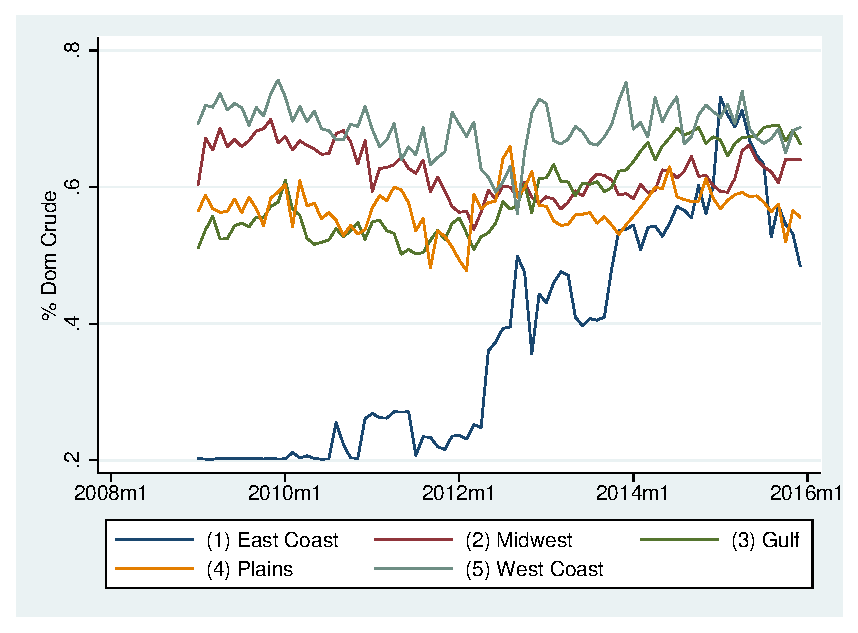
\includegraphics[width=0.65\textwidth]{\figpath/draft/avg_frac_dom_crude.eps}
\end{figure}

The primary explanation for low substitution towards domestic inputs is that crude oils are highly differentiated, and refineries are finely tuned to process a particular type of crude, although some refineries are vertically integrated with international oil companies like Citgo (Venezuela) or Aramco (Saudi Arabia).

As a result of this input differentiation and decades of costly investment, refineries are highly tailored to process specific crudes. Substantial changes to the crude slate require either months of reconfiguration or large capital changes. This is important, because the fracking boom has largely increased domestic supply of ``light'' (low density) crudes. Figure 1d shows the price domestic oil producers of ``light'' crude received, less the contemporaneous amount received by producers of ``heavy'' crude. Historically, lighter crudes traded at a premium, since they have larger naturally occurring shares of valuable end products. However, from 2010-2015, this long standing ordering was reversed, with the most valuable input trading at a substantial discount.

\subsection{Fracking Boom Regressions \label{sec:shaleRegression}}
We document that location and technological sophistication, which were determined before fracking transformed the U.S. oil market, correlated strongly with the extent to which firms benefited from the fracking boom. To do this, we first split the sample into a "pre" fracking period, prior to 2008, and a "post" fracking period, beginning in 2010.  For simplicity we exclude 2008 and 2009 from this "pre"-"post" analysis, although the results are similar with them included.

We calculate "pre" period average crude density (API), domestic crude share, size and technology (``downstream capacity'') for each refinery. These pre-period averages are interacted with an indictor for the post-period, as are indicators for which region the refinery is in (excluding PADD 1). Finally, we project monthly crude price paid by each firm onto these interacted variables, along with firm and month-of-sample dummies.

\begin{equation}
  CrudePrice_{ft}= 1\{Post_t\}\bar{X}^{pre}_{f}\beta + \nu_{f} + \mu_t +\epsilon_{ft} \label{eq:boomHeterogeneity}
\end{equation}

Table \ref{tab:within_PADD_winners} presents the results. Consistent with the exposition above, refineries proximate to shale deposits in the Midwest and Plains states saw large declines in crude costs relative to the omitted group, the East Coast. However, geography alone does not tell the whole story. Refineries processing "light" (high API gravity) crude in the pre-period, or with the technological capability to more easily switch between crudes, experienced larger gains. This regression confirms that pre-period factors like location and the type of crude a refinery is designed for, which were chosen before the shale boom, determined which refineries benefited. This panel variation underpins the identification strategy employed in the paper.

\begin{table}[]
  \centering
  \caption{Within-PADD Fracking Boom Beneficiaries \label{tab:within_PADD_winners}}
  {
\def\sym#1{\ifmmode^{#1}\else\(^{#1}\)\fi}
\begin{tabular}{l*{1}{c}}
\toprule
\midrule
API Gravity     & -0.00743** \\
                &(0.00294)   \\
\addlinespace
\% Domestic Crude&   -0.101***\\
                & (0.0376)   \\
\addlinespace
Log(Capacity)   & 0.000155   \\
                & (0.0123)   \\
\addlinespace
Downstream Capacity&  -0.0673*  \\
                & (0.0359)   \\
\addlinespace
(P2) Midwest    &   -0.116*  \\
                & (0.0597)   \\
\addlinespace
(P3) Gulf       &   0.0557   \\
                & (0.0632)   \\
\addlinespace
(P4) Plains     &   -0.173***\\
                & (0.0613)   \\
\addlinespace
(P5) West Coast &   0.0758   \\
                & (0.0661)   \\
\midrule
N               &     7653   \\
r2              &    0.958   \\
\bottomrule
\end{tabular}
}
 \\[1ex]
\begin{minipage}{.6\linewidth}
\scriptsize
  The dependent variable is the crude price paid  (\$/gal). All models contain firm-PADD fixed effects and month of sample dummies. The presented coefficients are the average pre-2008 values interacted with an indicator for the post boom period (post 2009). Years 2008 and 2009 are omitted. The sample is restricted to firms with at least 24 months of observations in both periods. Standard errors, clustered at the firm-PADD level, presented in parentheses.
\end{minipage}
\end{table}

\section{Supplementary Analysis }

\setcounter{table}{0} \renewcommand{\thetable}{\Alph{section}.\arabic{table}}
\setcounter{figure}{0} \renewcommand{\thefigure}{\Alph{section}.\arabic{figure}}

\subsection{Inputs Costs and the WTI Spot Price \label{App:wti_average_crude_cost}}
To evaluate whether the average input costs reported by refineries reflect marginal costs, we compare input costs to our closest observable proxy for marginal costs, the West Texas Intermediate Spot Price.  If long-run contracts that are not-indexed to spot prices dominate firms' crude acquisition, we would expect a relatively weak link between average input costs and spot prices.  In contrast, if firms acquire crude entirely on the spot market or through long-run contracts indexed to the spot price, we would expect high correlation between the two price series - in which case, average crude costs might offer a close approximation to marginal crude costs.

Comparing average input costs and WTI crude costs, we find evidence that the two move in concert - consistent with average crude costs being a relatively good proxy for marginal costs.  As a graphical illustration, Figure \ref{fig:input_costs_v_WTI}  plots U.S. average crude costs for all (composite), domestic and international crude streams against WTI crude spot price.  More formally, we can empirical test whether changes in average input costs are closely correlated with crude spot prices.  Table \ref{tab:input_costs_v_WTI} presents the coefficients from regressing first-differenced average input costs against contemporaneous and lagged first-differenced crude spot prices.  Consistent with the graphical evidence, we find changes in input costs are correlated with 80 percent of contemporaneous changes in spot prices and effectively 100 percent of changes in spot prices, after including the first lagged month.
\begin{figure}[]
\begin{centering}
\caption{Average Input Crude Costs and WTI Spot Prices, by Source \label{fig:input_costs_v_WTI}}
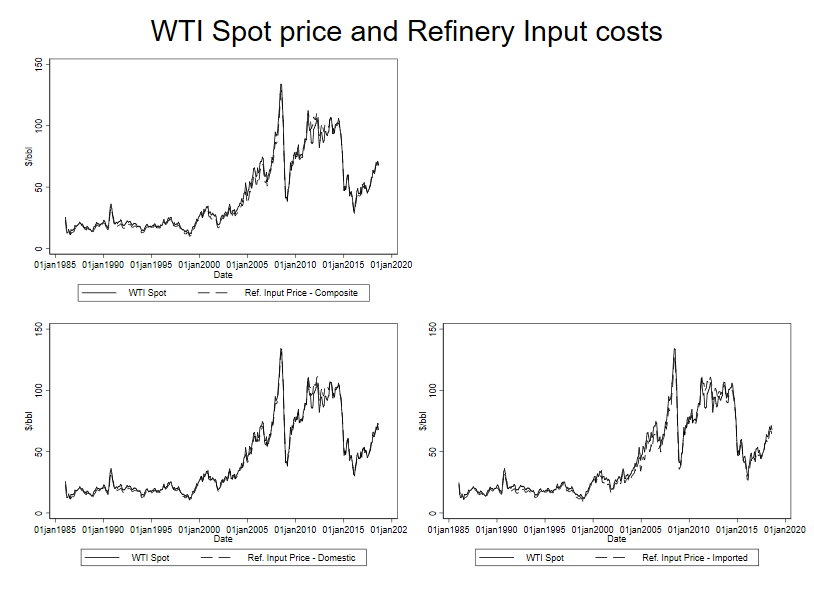
\includegraphics[width=0.7\textwidth]{\figpath/from_public_data/WTI_Spot_Input_Price.png}
\par\end{centering}
\vspace{4pt}
\scriptsize
\end{figure}

\begin{table}[]
\centering
\caption{Average Input Costs and WTI Spot Prices, by Source \label{tab:input_costs_v_WTI}}
{
\def\sym#1{\ifmmode^{#1}\else\(^{#1}\)\fi}
\begin{tabular}{l*{3}{c}}
\toprule
                    &\multicolumn{1}{c}{(1)}&\multicolumn{1}{c}{(2)}&\multicolumn{1}{c}{(3)}\\
                    &\multicolumn{1}{c}{Composite}&\multicolumn{1}{c}{Domestic}&\multicolumn{1}{c}{Imported}\\
\midrule
$\Delta WTISpot_t$  &        0.80\sym{***}&        0.76\sym{***}&        0.81\sym{***}\\
                    &     (0.012)         &     (0.013)         &     (0.019)         \\
$\Delta WTISpot_{t-1}$&        0.17\sym{***}&        0.22\sym{***}&        0.15\sym{***}\\
                    &     (0.018)         &     (0.018)         &     (0.022)         \\
$\Delta WTISpot_{t-2}$&      0.0046         &       0.019         &     -0.0020         \\
                    &     (0.013)         &     (0.015)         &     (0.019)         \\
$\Delta WTISpot_{t-3}$&      -0.016         &      -0.025\sym{**} &      -0.013         \\
                    &     (0.014)         &     (0.011)         &     (0.019)         \\
$\Delta WTISpot_{t-4}$&      -0.030\sym{*}  &       0.010         &      -0.054\sym{***}\\
                    &     (0.015)         &     (0.016)         &     (0.020)         \\
Constant            &       0.012         &       0.015         &      0.0033         \\
                    &     (0.038)         &     (0.039)         &     (0.052)         \\
\midrule
Observations        &         387         &         387         &         387         \\
R-Squared           &        0.96         &        0.96         &        0.93         \\
\bottomrule
\end{tabular}
}
 \\[1ex]
\smallskip{}
\begin{minipage}{.8\linewidth}
\scriptsize
Notes: Dependent variables in Cols 1 - 3 are the average nationwide refinery costs
	of input from all, domestic and imported sources, respectively.
\end{minipage}
\end{table}

\subsection{Instrumental Variables \label{App:IV}}

Based on the preceding discussion on refinery heterogeniety (Appendix \ref{App:Background}) and the fracking boom (Appendix \ref{App:ShaleBoom}), we construct four instrumental variables at the firm-month level.

The first two leverage cross-sectional differences in the type of crude oil refineries use. The logic of these instruments is similar to \cite{bartik_who_1991}.

\begin{description}
  \item[Gravity-based index price ($API$) -] The single biggest driver of price differentials across different crudes is oil density, measured by API gravity. As was discussed in Section \ref{App:Background}, refineries are configured to process a specific crude density, and deviate little from that in the data.

  The EIA reports monthly average delivered crude prices by API gravity, binned into five degree intervals. We calculate the average API for each refinery over the sample, and instrument using the price of the corresponding bin in the EIA data each month.

  \item[Index price interacted with downstream technology ($API-Downstream$) -] All refineries contain the same basic technology. However, many supplement this with additional ``downstream'' technology, which provides the refinery a moderate amount of flexibility in transforming a given crude into different end products. For this instrument, we construct the ratio of this downstream technology and distillation capacity (this ratio ranges from 0 to slightly above 2), and then interact this ratio with the $API$ instrument.

\end{description}

In addition to these instruments based on heterogeneity in refinery design, we also construct two instruments based on refinery location. As was discussed in Section 3, due to transportation constraints, the large price declines resulting from the shale boom were concentrated primarily in PADD's 2 and 4.  Following a similar logic, we interact time invariant indicators for whether a refinery is in one of these two regions, with time-varying price spread measures.

\begin{description}
  \item[WTI - Brent spot differential ($PADD 2,4-WTI$) -] This instrument interacts the US-Global spot price differential with an indicator for being in PADD 2 or 4. As shown in Figure 1b, this difference was small historically, but opened up to unprecedented levels during the shale boom.

  \item[US Heavy - Light Crude Spread ($PADD 2,4-HL$) -] This instrument interacts the US average difference between heavy and light crudes with an indicator for being in PADD 2 or 4. As shown in Figure 1d, this hedonic relationship was reversed during the shale boom, due to the light quality of shale oil.

\end{description}

These own cost instruments are created for every firm-month. We then construct instruments for rival and fringe competitors' costs analogously, by aggregating these own cost measures using the same weighting function employed in each rival and fringe cost calculation.

In sum, this generates eight instruments in the specifications which include own and rival costs as endogenous explanatory variables, and twelve instruments in models which separate out direct rival and fringe firm costs. Tables \ref{tab:iv_first_st} and \ref{tab:iv_first_fp} present the first stage results from columns (3) and (4) in Table 2. In general, the coefficients have sensible signs, and magnitudes, particularly comparing across columns. As the API instrument is a price index designed to track each refinery's crude type, a perfect index would have a coefficient close to one. Here the estimated coefficients are all large, but range from 0.65 for own costs, 0.85 for rival costs, and nearly 1 for fringe costs, suggesting measurement error at the individual refinery level. The downstream instrument is actually small in magnitude, and generally not significantly. However, as expected, the two geographic based instruments are large and significant, suggesting refineries in the midwest and plains states capture a large share of deviations in these benchmark differentials.

\begin{table}[]
 \centering
    \caption{Instrumental Variables First Stage - State Level \label{tab:iv_first_st}}
  \footnotesize
  {
\def\sym#1{\ifmmode^{#1}\else\(^{#1}\)\fi}
\begin{tabular}{l*{5}{c}}
\toprule
                &\multicolumn{1}{c}{(1)}   &\multicolumn{1}{c}{(2)}   &\multicolumn{1}{c}{(3)}   &\multicolumn{1}{c}{(4)}   &\multicolumn{1}{c}{(5)}   \\
\midrule
Own: API        &    0.641***& -0.00223   &    0.629***& -0.00309   & -0.00235   \\
                & (0.0253)   &(0.00550)   & (0.0252)   &(0.00684)   &(0.00589)   \\
\addlinespace
Own: API-Downstream&   0.0118   &  0.00340*  &   0.0124*  &  0.00667** & -0.00519***\\
                &(0.00731)   &(0.00201)   &(0.00735)   &(0.00264)   &(0.00190)   \\
\addlinespace
Own: PADD 2,4-HL&    0.444***& -0.00583   &    0.440***&  0.00857   & 0.000231   \\
                & (0.0241)   &(0.00452)   & (0.0239)   &(0.00846)   &(0.00543)   \\
\addlinespace
Own: PADD 2,4-WTI&    0.404***&  0.00945*  &    0.405***&  -0.0172** &  0.00693   \\
                & (0.0255)   &(0.00508)   & (0.0252)   &(0.00758)   &(0.00473)   \\
\addlinespace
Rival: API      &    0.205***&    0.847***&    0.175***&    0.819***&  -0.0348***\\
                & (0.0300)   & (0.0108)   & (0.0354)   & (0.0171)   & (0.0102)   \\
\addlinespace
Rival: API-Downstream& 0.000453   &  -0.0319***&   0.0331***&   0.0309***& -0.00624** \\
                & (0.0235)   &(0.00810)   & (0.0116)   &(0.00698)   &(0.00314)   \\
\addlinespace
Rival: PADD 2,4-HL&   -0.187***&    0.314***&   -0.122** &    0.203***&   0.0467***\\
                & (0.0527)   &(0.00854)   & (0.0507)   & (0.0206)   &(0.00998)   \\
\addlinespace
Rival: PADD 2,4-WTI&    0.106** &    0.489***&   0.0430   &    0.565***&   0.0142*  \\
                & (0.0464)   & (0.0114)   & (0.0359)   & (0.0167)   &(0.00847)   \\
\addlinespace
Fringe: API     &            &            &   0.0438   &   0.0273*  &    0.958***\\
                &            &            & (0.0408)   & (0.0151)   & (0.0115)   \\
\addlinespace
Fringe: API-Downstream&            &            &  -0.0176   &  -0.0257***&  -0.0770***\\
                &            &            & (0.0149)   &(0.00473)   &(0.00480)   \\
\addlinespace
Fringe: PADD 2,4-HL&            &            &  -0.0692   &   0.0364   &    0.215***\\
                &            &            & (0.0630)   & (0.0223)   & (0.0130)   \\
\addlinespace
Fringe: PADD 2,4-WTI&            &            &   0.0293   &-0.000599   &    0.319***\\
                &            &            & (0.0537)   & (0.0200)   & (0.0155)   \\
\midrule
Rival Measure   &            &            &      Avg   &      Avg   &      Avg   \\
Endogenous Var  &      Own   &    Rival   &      Own   &    Rival   &   Fringe   \\
N               &    71570   &    71570   &    71529   &    71529   &    71529   \\
r2              &    0.975   &    0.997   &    0.975   &    0.995   &    0.997   \\
\bottomrule
\end{tabular}
}
 \\[1ex]
  \begin{minipage}{\linewidth}
  \scriptsize
  This table presents the first stage results from the state level instrumental variable regressions presented in panel (a) of Table 2. Models (1)-(2) contain the first stage results for the three crude cost variables in the second stage model with month of sample fixed effects (regression 6 from Table 2), and models (3)-(4) contain the first stage results for the second stage model with month and year fixed effects (regression 7 from Table 2). The rows list the excluded variables from each regression, with ``Domestic'' referring to the domestic crude share instrument, and ``API'' referring to the API gravity instrument. These are averaged over rival and non-rival firms to match the structure of these variables in the second stage.
  \end{minipage}
\end{table}

\begin{table}[]
  \centering
    \caption{Instrumental Variables First Stage - Firm Level \label{tab:iv_first_fp}}
  \footnotesize
  {
\def\sym#1{\ifmmode^{#1}\else\(^{#1}\)\fi}
\begin{tabular}{l*{5}{c}}
\toprule
                &\multicolumn{1}{c}{(1)}   &\multicolumn{1}{c}{(2)}   &\multicolumn{1}{c}{(3)}   &\multicolumn{1}{c}{(4)}   &\multicolumn{1}{c}{(5)}   \\
\midrule
Own: API        &    0.619***&   0.0178   &    0.597***& 0.000388   &  -0.0306   \\
                & (0.0845)   & (0.0153)   & (0.0876)   & (0.0172)   & (0.0194)   \\
\addlinespace
Own: API-Downstream&  0.00224   &  0.00294   &  0.00555   &  0.00658   &-0.000777   \\
                & (0.0172)   &(0.00407)   & (0.0164)   &(0.00473)   &(0.00352)   \\
\addlinespace
Own: PADD 2,4-HL&    0.406***&   0.0257   &    0.381***&   0.0239   &   0.0250   \\
                & (0.0896)   & (0.0225)   & (0.0974)   & (0.0314)   & (0.0252)   \\
\addlinespace
Own: PADD 2,4-WTI&    0.200** &  0.00612   &    0.184** &  -0.0361   & -0.00335   \\
                & (0.0980)   & (0.0228)   & (0.0755)   & (0.0379)   & (0.0181)   \\
\addlinespace
Rival: API      &   0.0795   &    0.841***&    0.103   &    0.862***&   -0.112***\\
                & (0.0748)   & (0.0300)   &  (0.163)   & (0.0431)   & (0.0308)   \\
\addlinespace
Rival: API-Downstream&   0.0568   &  -0.0318*  &    0.132** &   0.0692***&  -0.0499***\\
                & (0.0694)   & (0.0188)   & (0.0607)   & (0.0208)   & (0.0131)   \\
\addlinespace
Rival: PADD 2,4-HL&   -0.108   &    0.219***&  -0.0817   &    0.129*  &   0.0730   \\
                &  (0.216)   & (0.0449)   &  (0.243)   & (0.0662)   & (0.0452)   \\
\addlinespace
Rival: PADD 2,4-WTI&    0.540***&    0.500***&    0.441***&    0.604***&  -0.0652*  \\
                &  (0.196)   & (0.0528)   &  (0.143)   & (0.0773)   & (0.0380)   \\
\addlinespace
Fringe: API     &            &            &  -0.0237   &  -0.0162   &    1.111***\\
                &            &            &  (0.163)   & (0.0282)   & (0.0322)   \\
\addlinespace
Fringe: API-Downstream&            &            &  -0.0114   & -0.00820   &  -0.0666***\\
                &            &            & (0.0362)   &(0.00641)   &(0.00877)   \\
\addlinespace
Fringe: PADD 2,4-HL&            &            &    0.153   &    0.156***&    0.154***\\
                &            &            &  (0.195)   & (0.0403)   & (0.0566)   \\
\addlinespace
Fringe: PADD 2,4-WTI&            &            &  -0.0528   &  -0.0851***&    0.366***\\
                &            &            &  (0.153)   & (0.0320)   & (0.0361)   \\
\midrule
Rival Measure   &            &            &      Avg   &      Avg   &      Avg   \\
Endogenous Var  &      Own   &    Rival   &      Own   &    Rival   &   Fringe   \\
N               &     9169   &     9169   &     9169   &     9169   &     9169   \\
r2              &    0.969   &    0.997   &    0.969   &    0.996   &    0.995   \\
\bottomrule
\end{tabular}
}
 \\[1ex]
  \begin{minipage}{\linewidth}
  \scriptsize
  This table presents the first stage results from the firm-PADD level instrumental variable regressions presented in panel (b) of Table 2. Models (1)-(2) contain the first stage results for the three crude cost variables in the second stage model with month of sample fixed effects (regression 6 from Table 2), and models (3)-(4) contain the first stage results for the second stage model with month and year fixed effects (regression 7 from Table 2). The rows list the excluded variables from each regression, with ``Domestic'' referring to the domestic crude share instrument, and ``API'' referring to the API gravity instrument. These are averaged over rival and non-rival firms to match the structure of these variables in the second stage.
  \end{minipage}
\end{table}

\subsection{Alternative Rival Definitions  \label{App:RivalDefs}}

In our main specification, rival costs enter as the inverse shipping cost weighted average of competing firms. In this appendix, we consider two alternatives. First, rather than using shipping cost, we also consider simple inverse linear distance between refineries. Those results are presented in columns 1 and 3 of Table \ref{tab:RivalComp_Max}.

In some markets, such as electricity, strict capacity constraints and heterogeneous costs impose a natural ``dispatch'' ordering across firms. In these situations, the market price is set by the cost of the ``marginal firm'', rather than the average over inframarginal firms serving a market. Such a simple dispatch model does not well describe refinery competition, where capacity constraints are less stark and storage is possible. Nevertheless, we estimate a dispatch-curve model in this setting, replacing the average of rival costs with the contemporaneous cost of the rival which is highest cost on average in the other months during the same year. These results are presented in columns 2 and 4.

\begin{sidewaystable}[h!]
  \centering
    \caption{Competition measure results \label{tab:RivalComp_Max}}
  \footnotesize
    \subfloat[State Level Results]{{
\def\sym#1{\ifmmode^{#1}\else\(^{#1}\)\fi}
\begin{tabular}{l*{4}{c}}
\toprule
                &\multicolumn{1}{c}{(1)}   &\multicolumn{1}{c}{(2)}   &\multicolumn{1}{c}{(3)}   &\multicolumn{1}{c}{(4)}   \\
\midrule
Own             &   0.0513***&   0.0562***&   0.0705***&   0.0476** \\
                & (0.0131)   & (0.0132)   & (0.0248)   & (0.0237)   \\
\addlinespace
Rival           &   0.0854***&   0.0435***&  0.00624   &    0.118***\\
                & (0.0171)   & (0.0109)   & (0.0313)   & (0.0272)   \\
\addlinespace
Fringe          &    0.196***&    0.253***&    0.146***&   0.0820***\\
                & (0.0195)   & (0.0159)   & (0.0311)   & (0.0286)   \\
\addlinespace
Brent Spot      &    0.620***&    0.601***&    0.718***&    0.691***\\
                & (0.0102)   & (0.0102)   & (0.0107)   & (0.0116)   \\
\midrule
Rival Measure   &   AvDist   &      Max   &   AvDist   &      Max   \\
IV              &            &            &      Yes   &      Yes   \\
fstat           &            &            &     3041   &     1339   \\
N               &    71529   &    71517   &    71529   &    71517   \\
\bottomrule
\end{tabular}
}
} \subfloat[Firm Level Results]{{
\def\sym#1{\ifmmode^{#1}\else\(^{#1}\)\fi}
\begin{tabular}{l*{4}{c}}
\toprule
                &\multicolumn{1}{c}{(1)}   &\multicolumn{1}{c}{(2)}   &\multicolumn{1}{c}{(3)}   &\multicolumn{1}{c}{(4)}   \\
\midrule
Own             &   0.0508*  &   0.0782***&  -0.0252   &  0.00687   \\
                & (0.0298)   & (0.0269)   & (0.0707)   & (0.0435)   \\
\addlinespace
Rival           &    0.171***&    0.105***&    0.165   &    0.247***\\
                & (0.0369)   & (0.0238)   &  (0.106)   & (0.0710)   \\
\addlinespace
Fringe          &   0.0907** &    0.150***&   0.0479   &  -0.0256   \\
                & (0.0351)   & (0.0321)   & (0.0599)   & (0.0559)   \\
\addlinespace
Brent Spot      &    0.642***&    0.621***&    0.752***&    0.707***\\
                & (0.0159)   & (0.0185)   & (0.0231)   & (0.0273)   \\
\midrule
Rival Measure   &   AvDist   &      Max   &   AvDist   &      Max   \\
IV              &            &            &      Yes   &      Yes   \\
First-stage F   &            &            &      123   &      167   \\
N               &     9169   &     9169   &     9169   &     9169   \\
\bottomrule
\end{tabular}
}
} \\
  \begin{minipage}{\linewidth}
  \scriptsize
    This table presents the results of estimating Equation (3) using total average wholesale prices as the dependent variable. Panel (a) is estimated at the firm-state-month level, and includes firm-state fixed effects; Panel (b) is estimated at the firm-PADD-month level and includes firm-PADD fixed effects. All specifications include year fixed effect and month fixed effects.  Rival costs include the average crude price of other firms selling into the same market each month, and non-rival costs are the average cost of all other firms, weighted by the inverse shipping cost of supplying the market. Standard errors are presented in parentheses, clustered at the firm-state level in panel (a) and the firm level in panel (b). All models include demand shifters (state population, income, heating and cooling degree days) and supply shifters (diesel and gasoline shares, proportion of retail sales, API gravity, and operating refinery capacity).
\end{minipage}
\end{sidewaystable}

\subsection{Heterogeneity}

The models in the text estimate a single average reduced-form pass-through rate for the entire industry. Structurally, we know that pass-through varies with the relative convexity of residual demand and supply \citep{weyl_pass-through_2013}. Mapping these to observed market structure requires assumptions about the nature of competition. Nevertheless, we can check if average pass-through varies with observables likely correlated with these factors.

Table \ref{tab:RivalComp_Heterogeneity} presents the results from models 1 and 3 from Table 2 with the main pass-through terms interacted with correlates for market structure. In models 1 and 3, pass-through is interacted with an indicator for whether the average HHI for that market during other months in the same year is above the median for the sample. In models 2 and 4, the interaction term is an indicator for whether the firm had more than a 10 percent share of refining capacity in that PADD at the start of the year.

\begin{sidewaystable}[h!]
  \centering
    \caption{Competition measure results \label{tab:RivalComp_Heterogeneity}}
  \footnotesize
    \subfloat[State Level Results]{{
\def\sym#1{\ifmmode^{#1}\else\(^{#1}\)\fi}
\begin{tabular}{l*{4}{c}}
\toprule
                &\multicolumn{1}{c}{(1)}   &\multicolumn{1}{c}{(2)}   &\multicolumn{1}{c}{(3)}   &\multicolumn{1}{c}{(4)}   \\
\midrule
Own             &   0.0445** &   0.0373** &   0.0478   &   0.0348   \\
                & (0.0180)   & (0.0171)   & (0.0320)   & (0.0369)   \\
\addlinespace
Own X Int       & 0.000282   &   0.0286   &   0.0273   &   0.0549   \\
                & (0.0211)   & (0.0289)   & (0.0382)   & (0.0600)   \\
\addlinespace
Rival           &    0.282***&    0.295***&    0.157***&    0.181***\\
                & (0.0200)   & (0.0214)   & (0.0354)   & (0.0452)   \\
\addlinespace
Rival X Int     & -0.00213   &  -0.0418   &  -0.0299   &  -0.0685   \\
                & (0.0213)   & (0.0307)   & (0.0384)   & (0.0618)   \\
\addlinespace
Brent Spot      &    0.626***&    0.625***&    0.734***&    0.729***\\
                & (0.0112)   & (0.0115)   & (0.0124)   & (0.0134)   \\
\midrule
Interaction     &      HHI   & Cap.PADD   &      HHI   & Cap.PADD   \\
Time FE         &      Y,M   &      Y,M   &      Y,M   &      Y,M   \\
IV              &            &            &      Yes   &      Yes   \\
fstat           &            &            &     2329   &     1551   \\
N               &    71570   &    71570   &    71570   &    71570   \\
\bottomrule
\end{tabular}
}
}
    \subfloat[Firm Level Results]{{
\def\sym#1{\ifmmode^{#1}\else\(^{#1}\)\fi}
\begin{tabular}{l*{4}{c}}
\toprule
                &\multicolumn{1}{c}{(1)}   &\multicolumn{1}{c}{(2)}   &\multicolumn{1}{c}{(3)}   &\multicolumn{1}{c}{(4)}   \\
\midrule
Own             &   0.0486   &   0.0368   &  -0.0433   &  -0.0822   \\
                & (0.0400)   & (0.0369)   & (0.0624)   & (0.0677)   \\
\addlinespace
Own X Int       &  0.00100   &   0.0795   &    0.136   &    0.243***\\
                & (0.0406)   & (0.0572)   & (0.0860)   & (0.0825)   \\
\addlinespace
Rival           &    0.285***&    0.306***&    0.238***&    0.309***\\
                & (0.0444)   & (0.0402)   & (0.0741)   & (0.0810)   \\
\addlinespace
Rival X Int     & -0.00189   &   -0.105*  &   -0.137   &   -0.268***\\
                & (0.0386)   & (0.0559)   & (0.0845)   & (0.0821)   \\
\addlinespace
Brent Spot      &    0.622***&    0.619***&    0.747***&    0.722***\\
                & (0.0176)   & (0.0180)   & (0.0242)   & (0.0246)   \\
\midrule
Interaction     &      HHI   & Cap.PADD   &      HHI   & Cap.PADD   \\
Time FE         &      Y,M   &      Y,M   &      Y,M   &      Y,M   \\
IV              &            &            &      Yes   &      Yes   \\
fstat           &            &            &      120   &      114   \\
N               &     9169   &     9169   &     9169   &     9169   \\
\bottomrule
\end{tabular}
}
} \\
    \smallskip{}
  \begin{minipage}{.9\linewidth}
  \scriptsize
   This table presents the results of estimating Equation (3) using total average wholesale prices as the dependent variable. Panel (a) is estimated at the firm-state-month level, and includes firm-state fixed effects; Panel (b) is estimated at the firm-PADD-month level and includes firm-PADD fixed effects. All specifications include year fixed effect and month fixed effects. ``X Int'' variables reflect the cost measure listed, interacted with a binary indictor based on the measure listed in the Interaction row. Standard errors are presented in parentheses, clustered at the firm-state level. All models include demand shifters and supply shifters.
  \end{minipage}
\end{sidewaystable}
\clearpage
\subsection{Carbon Tax}

\begin{figure}[H]
\centering
\caption{GHG heterogeneity \label{fig:ghg_histogram}}
\includegraphics[width=0.7\textwidth]{../output/from_server/figures/hist_co2e_refinery} \\
\vspace{4pt}
\begin{minipage}{.6\linewidth}
\scriptsize
Based on annual data (2011-2015) in EPA GHGRP.
\end{minipage}
\end{figure}

\begin{table}[H]
\centering
\caption{Determinants of CO2 Heterogeneity \label{tab:co2_reg}}
\input{../output/from_server/tables/co2e_regression_refinery.tex} \\
\vspace{4pt}
\begin{minipage}{.6\linewidth}
\scriptsize
Dependent variable: Metric tons of CO2 equivalent per barrel of inputs processed. Data from EPA GHGRP (2011-2015). Model includes PADD and year dummies.
\end{minipage}
\end{table}

\clearpage
\bibliographystyle{aer}
\bibliography{MS_passthrough}

\end{document}
